\documentclass[12]{article}
\usepackage[utf8]{inputenc}

%Packages

\usepackage{amsmath}
\usepackage{hyperref}
\usepackage{cleveref}
\usepackage{float}
\usepackage[margin=0.5in]{geometry}
\usepackage{graphicx}
\usepackage{multicol}
\usepackage{multirow}
\usepackage{siunitx}
\usepackage[numbib]{tocbibind}
\usepackage{import}
\usepackage{booktabs}
\usepackage{array}
\usepackage{gensymb}
\usepackage{bm}
\usepackage{minted}
\usepackage{sectsty}

%Preamble

\title{Using Gyroscopic Phenomena for Attitude Control \\ 3C5 Full Technical Report}
\author{Zach Lambert}
\date{08/12/19}
\makeatletter

\parindent 0pt
\parskip 10pt

\sisetup{
    round-mode = places,
    round-precision = 2,
}

%Main Document

\begin{document}

\begin{centering}
\huge{\@title}

\large{
\@author \\
Pembroke College \\
\@date
}

\end{centering}

\begin{multicols*}{2}

\section{Abstract}

The objective of this report was to investigate how gyroscopic phenomena can be utilised in spacecrafts for attitude control, as an interesting application of gyroscopes. This included reaction wheels, which use rotors with variable spin, and control moment gyroscopes, which use rotors with variable spin axes. In addition to deriving equations of motion that describe these systems and finding solutions, numerical integration was used to validate these and simulate less predictable behaviour. It was found that reaction wheels can control angular velocity along the same axis as the rotor by varying the rotor spin, although the solution become more complex when using 3 reaction wheels. On the other hand, control moment gyroscopes controlled angular velocity along an axis perpendicular to the spin axis, but can't sustain stable rotation for prolonged periods of time.

\section{Introduction}

This report investigates how gyroscopic phenomena can be used for attitude control in spacecrafts. The two actuators of interest are reaction wheels and control moment gyroscopes (CMGs), which are commonly used \cite{reaction_wheels} \cite{hubble}.

Both reaction wheels and CMGs exploit conservation of angular momentum to control the angular velocity of the spacecraft. By changing the angular momentum of gyroscopes within the spacecraft, the angular momentum of the whole spacecraft must experience an equal and opposite change, such that the total angular momentum remains constant \cite{device_explanation}.

Reaction wheels use spinning rotors with variable angular velocity. They change the angular velocity of the gyroscopes by changing the rotor spin, while the spin axis remains fixed relative to the spacecraft. 

Control moment gyroscopes utilise gyroscopic precession to rotate the spacecraft. They use rotors mounted in single gimbals, allowing the spin axis to be controlled about one axis, while the rotor operates at fixed spin. By tilting the spin axis of the rotor, this changes the angular momentum of the gyroscope.

The advantage of gyroscopic devices for attitude control over thrusters, is that they are driven by motors, which use electricity that can be generated by solar panels. On the other hand, thrusters use propellent which cannot be recovered.

\section{Method}

\subsection{Finding Analytical Solutions}

For each system investigated, the first step was to find the equations of motion. Following this, analytical solutions could be found for a variety of types of behaviour.

Additionally, by adding perturbations to the equilbrium solutions, the stability of solutions could be investigated.

\subsection{Validating Solutions with Numerical Integration}

In order to validate that the solutions found are sensible, as well as investigate more complex motion, numerical integration was used to integrate the equations of motion.

Since the equations of motion are all first order, a single application of the fourth-order Runge-Kutta formula (RK4) can be used, described below \cite{RK4}. \\
If the equations of motion can be described by $\dot{\bm{y}} = f(t, \bm{y})$, then $\bm{y}$ is integrated using this formula :
$$ \bm{y}(t_{n+1}) = \bm{y}(t_n) +
\frac{1}{6}(k_1 + 2k_2 + 2k_3 + k_4)\Delta t + O(\Delta t^5)$$
Where:
\begin{align*}
k_1 &= f(t_n, \bm{y}(t_n)) \\
k_2 &= f(t_n + \Delta t/2, \bm{y}(t_n) + k_1\Delta t/2) \\
k_3 &= f(t_n + \Delta t/2, \bm{y}(t_n) + k_2\Delta t/2) \\
k_4 &= f(t_n + \Delta t, \bm{y}(t_n) + k_3\Delta t)
\end{align*}

To check a given solution, the integrator needs to be supplied the function $f$ and the initial conditions.

The function $f$ includes time dependence because of properties of the system which can vary in time. For the reaction wheels, the rotor spins could vary, and for the control moment gyroscopes, the spin axis inclination could vary.

This was implemented in Python, the details of which can be seen in the appendix.

\vfill\null
\columnbreak

\section{Results}

\subsection{Motion of the Spacecraft with No Actuators}

\begin{figure}[H]
\centering
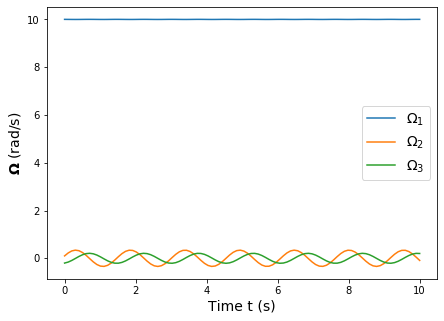
\includegraphics[width=0.9\linewidth]{fig/no_actuation_ABC_stable.png}
\vspace{-0.3cm}
\caption{\label{fig:no_actuation_ABC_stable}Stable motion of an ABC body with constant angular velocity about a principle axis. Stable motion occurs when this principle axis has the minimum or maximum moment of inertia}
\end{figure}

\begin{figure}[H]
\centering
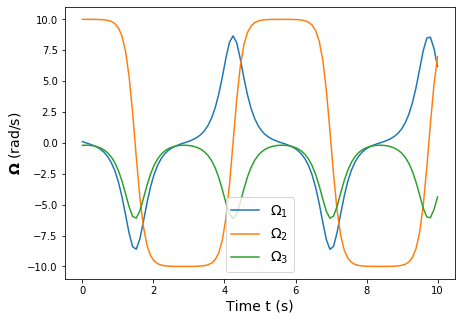
\includegraphics[width=0.9\linewidth]{fig/no_actuation_ABC_unstable.png}
\vspace{-0.3cm}
\caption{\label{fig:no_actuation_ABC_unstable}Unstable motion of an ABC body. Unstable motion occurs when the body attempts to rotate about the principle axis with intermediate moment of inertia.}
\end{figure}

\vfill\null
\columnbreak

\subsection{Motion of the Spacecraft with Reaction Wheels}

\begin{figure}[H]
\centering
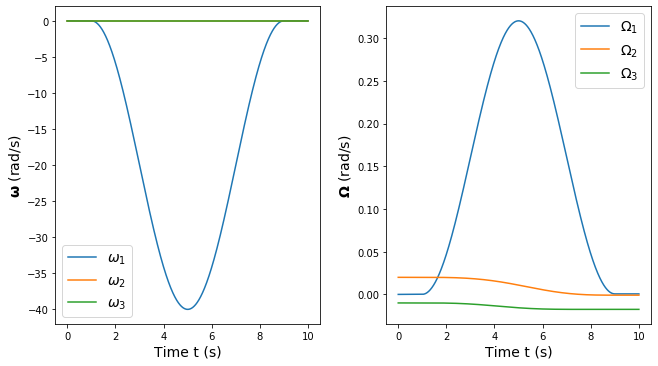
\includegraphics[width=\linewidth]{fig/reaction_single_zero_stable.png}
\vspace{-0.3cm}
\caption{\label{fig:reaction_single_zero_stable}Example of stable rotation about an axis using a single reaction wheel with variable spin. Perturbations in the other axes follow stable oscillation.}
\end{figure}

\begin{figure}[H]
\centering
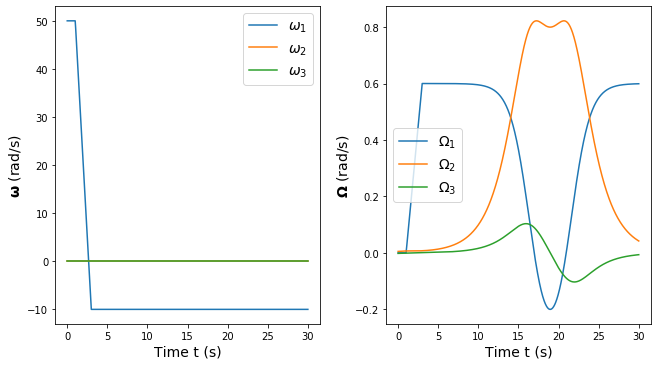
\includegraphics[width=\linewidth]{fig/reaction_single_zero_unstable.png}
\vspace{-0.3cm}
\caption{\label{fig:reaction_single_zero_unstable}Example of unstable rotation about a axis using a single reaction wheel with variable spin. Perturbations in the other axes grow exponentially and cause the motion to become unpredictable.}
\end{figure}

\begin{figure}[H]
\centering
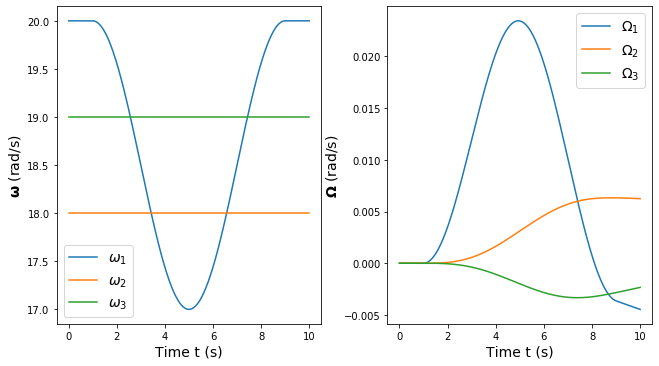
\includegraphics[width=\linewidth]{fig/reaction_naive_attempt.png}
\vspace{-0.3cm}
\caption{\label{fig:reaction_naive_attempt}Demonstrates what happens if there is attempted rotation about a axis using a single reaction wheel when the other reaction wheels are spinning too. In this case, the spin of the other reaction wheels need to be changed too.}
\end{figure}

\begin{figure}[H]
\centering
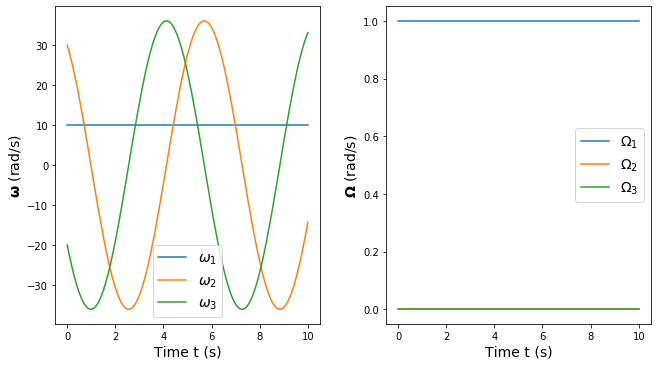
\includegraphics[width=\linewidth]{fig/reaction_smart_constant.png}
\vspace{-0.3cm}
\caption{\label{fig:reaction_smart_constant}Demonstrates the correct method of rotating about a single axis using reaction wheels when all the reaction wheels have spin. In this case, the spacecraft has constant angular velocity about an axis.}
\end{figure}

\begin{figure}[H]
\centering
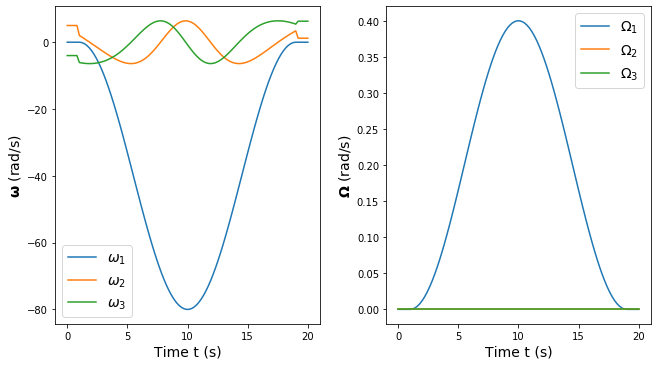
\includegraphics[width=\linewidth]{fig/reaction_smart_variable.png}
\vspace{-0.3cm}
\caption{\label{fig:reaction_smart_variable}Shows how reaction wheels can be used to rotate the spacecraft about a single axis with a varying angular velocity.}
\end{figure}

\subsection{Motion of the Spacecraft with Control Moment Gyroscopes}

\begin{figure}[H]
\centering
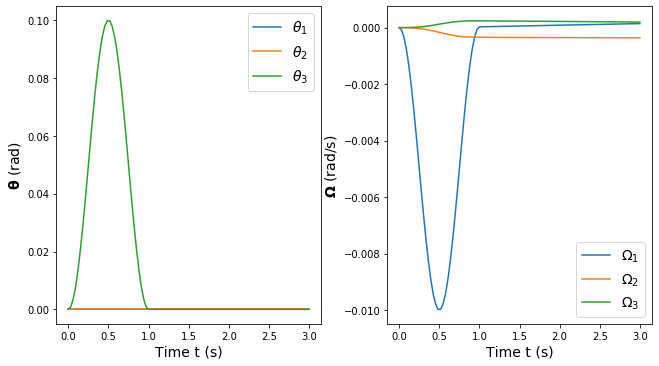
\includegraphics[width=\linewidth]{fig/cmg_controlled.png}
\vspace{-0.3cm}
\caption{\label{fig:cmg_controlled}Demonstrates how a set of control moment gyroscopes can be used to provide controlled rotation about an axis. In this case, the changes in angular velocity about the other two axes have been kept small, so don't affect the motion significantly. }
\end{figure}

\begin{figure}[H]
\centering
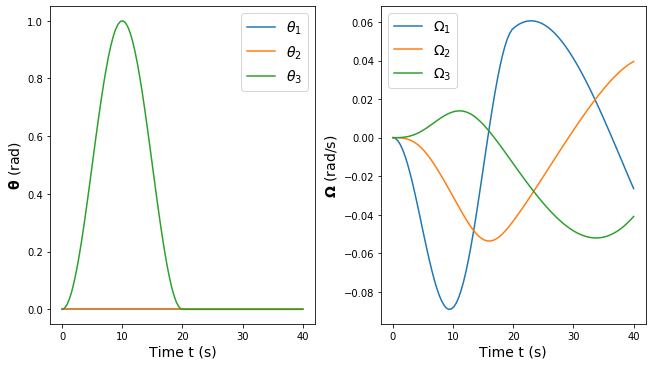
\includegraphics[width=\linewidth]{fig/cmg_uncontrolled.png}
\vspace{-0.3cm}
\caption{\label{fig:cmg_uncontrolled}Demonstrates how the the control moment gyroscopes can produce uncontrolled motion. In this case, the angular velocity about other axes was allowed to become too large, which caused the motion to become uncontrolled.}
\end{figure}

\vfill\null
\columnbreak

\section{Discussion}

\subsection{Motion of the Spacecraft with No Actuators}

\subsubsection{Equations of Motion}

Define $I$ as the inertia matrix of the spacecraft about the centre of mass and $\bm{\Omega}$ as its angular velocity. This means that the angular momentum about the centre of mass is given by \cite{inertia_matrix}:
\begin{equation} \label{eq:spacecraft_h}
\bm{h} = I\bm{\Omega}
\end{equation}
In order for this inertia matrix to be diagonal, therefore simplifying the analysis, vectors must be defined relative to the principle axis of the spacecraft, defined as $\bm{i}$, $\bm{j}$ and $\bm{k}$.

To find the equations of motions, we used the equation \cite{Q_equals_hdot}:
\begin{equation} \label{eq:general_eq_of_motion}
\bm{Q}_P = \bm{\dot{h}}_P + \bm{r}_P\times \bm{p}
\end{equation}

However, since angular momentum is taken about the centre of mass ($\bm{r}_P \times \bm{p} = 0$), this simplifies to:
\begin{equation} \label{eq:simple_eq_of_motion}
\bm{Q} = \bm{\dot{h}}
\end{equation}

This is only valid if $\dot{\bm{h}}$ is defined within a fixed reference frame. However the expression for $\bm{h}$ given in \cref{eq:spacecraft_h} is defined in the reference frame of the spacecraft, which is rotating with angular velocity $\Omega$. To evaluate $\bm{\dot{h}}$ in a fixed reference frame $F$, when defined in a rotating reference frame $R$, the following is used \cite{dif_rotating_frame}:
\begin{equation} \label{eq:dif_rotating_frame}
\left[ \dot{\bm{h}} \right]_F = \left[ \dot{\bm{h}} \right]_R + \bm{\Omega}\times \left[ \bm{h} \right]_R
\end{equation}

Combining \cref{eq:spacecraft_h}, \cref{eq:general_eq_of_motion} and \cref{eq:dif_rotating_frame} gives:
\begin{equation} \label{eq:euler_equations_vector}
\bm{Q} = \dot{\bm{h}} = I\bm{\dot{\Omega}} + \bm{\Omega}\times I\bm{\Omega}
\end{equation}

Expanding this out gives the equations of motion for the spacecraft, which are Euler's equations:
\begin{align}
\label{eq:euler_equations}
\begin{split}
Q_1 &= A\dot{\Omega}_1 + (C - B)\Omega_2\Omega_3 \\
Q_2 &= B\dot{\Omega}_2 + (A - C)\Omega_1\Omega_3 \\
Q_3 &= C\dot{\Omega}_3 + (B - A)\Omega_1\Omega_2 \\
\end{split}
\end{align}

Since all the systems being investigated have no external torques, the $\bm{Q}$ will always be zero.

\subsubsection{Constant Angular Velocity Solution}

In order for the spacecraft to rotate about its axes, it will need to be able to rotate at constant angular velocity about its axes. From \cref{eq:euler_equations} it can be seen that having constant angular velocity about a single axis is a valid solution. For example, set $\bm{\Omega} = \Omega\bm{i} = \textrm{Constant}$ and $\bm{Q}=0$, then substitute into \cref{eq:euler_equations}:
\begin{align*}
0 &= 0 + (C - B)\times 0 \times 0 = 0 \\
0 &= 0 + (A - C)\times\Omega_1 \times 0 = 0 \\
0 &= 0 + (B - A)\times \Omega_1 \times 0 = 0 \\
\end{align*}

Therefore, in the absence of external couples, there can be constant motion about a single principle axis. However, only certain solutions are stable. To investigate stability, set $\Omega_2$ and $\Omega_3$ to have small perturbations:
\begin{equation} \label{eq:euler_stability_omega}
\bm{\Omega} =
\begin{pmatrix}
\Omega_1 \\
\delta\Omega_2 \\
\delta\Omega_3
\end{pmatrix}
\end{equation}
Substituting \cref{eq:euler_stability_omega} into \cref{eq:euler_equations} and ignoring second order terms of perturations gives:
\begin{align}
\label{eq:euler_stability_equations}
\begin{split}
0 &= A\dot{\Omega}_1 \\
0 &= B\delta\dot{\Omega}_2 + (A - C)\Omega_1\delta\Omega_3 \\
0 &= C\delta\dot{\Omega}_3 + (B - A)\Omega_1\delta\Omega_2 \\
\end{split}
\end{align}

From \cref{eq:euler_stability_equations} we get a pair of coupled first order equations for $\delta\Omega_2$ and $\delta\Omega_3$:
\begin{align}
\label{eq:euler_stability_first_order}
\begin{split}
\delta\dot{\Omega}_2 = \Omega_1\frac{C-A}{B}\delta\Omega_3 \\
\delta\dot{\Omega}_3 = -\Omega_1\frac{B-A}{C}\delta\Omega_2
\end{split}
\end{align}
These can be combined to give second order differential equations for $\delta\Omega_2$ and $\delta\Omega_3$.
\begin{align}
\label{eq:euler_stability_second_order}
\begin{split}
\delta\ddot{\Omega}_2 &= -\Omega_1^2\frac{(B-A)(C-A)}{BC}\delta\Omega_2 \\
\delta\ddot{\Omega}_3 &= -\Omega_1^2\frac{(B-A)(C-A)}{BC}\delta\Omega_3
\end{split}
\end{align}

The solutions to these equations are:
\begin{equation} \label{eq:euler_stability_solution}
\delta\Omega_2 = k\sin{(\omega t + \phi)} \quad\quad
\delta\Omega_3 = k\cos{(\omega t + \phi)}
\end{equation}
Where $A$ and $\phi$ depend on initial conditions, and:
\begin{equation} \label{eq:euler_stability_frequency}
\omega^2 = \Omega_1^2\frac{(B-A)(C-A)}{BC}
\end{equation}

In order for this to be a valid solution and therefore be stable, $\omega^2$ must be positive. Otherwise, $\delta\Omega_2$ and $\delta\Omega_3$ will grow exponentially and be unstable. In the case that $A<B<C$, $\omega^2$ will be positive when rotating about the $\bm{i}$ or $\bm{k}$ axis, but negative for the $\bm{j}$ axis. Therefore, the body can have stable rotation about its principle axis with the minimum or maximum moment of inertia, but not the intermediate moment of inertia.

For constant angular velocity of an ABC body about a principle axis, \Cref{fig:no_actuation_ABC_stable} shows the results of a simulation about a stable axis and \Cref{fig:no_actuation_ABC_unstable} shows the results of a simulation about an unstable axis, when the other components of angular velocity have been given small perturbations.

\subsection{Motion of the Spacecraft with Reaction Wheels}

\subsubsection{Structure of the System}

\begin{figure}[H]
\centering
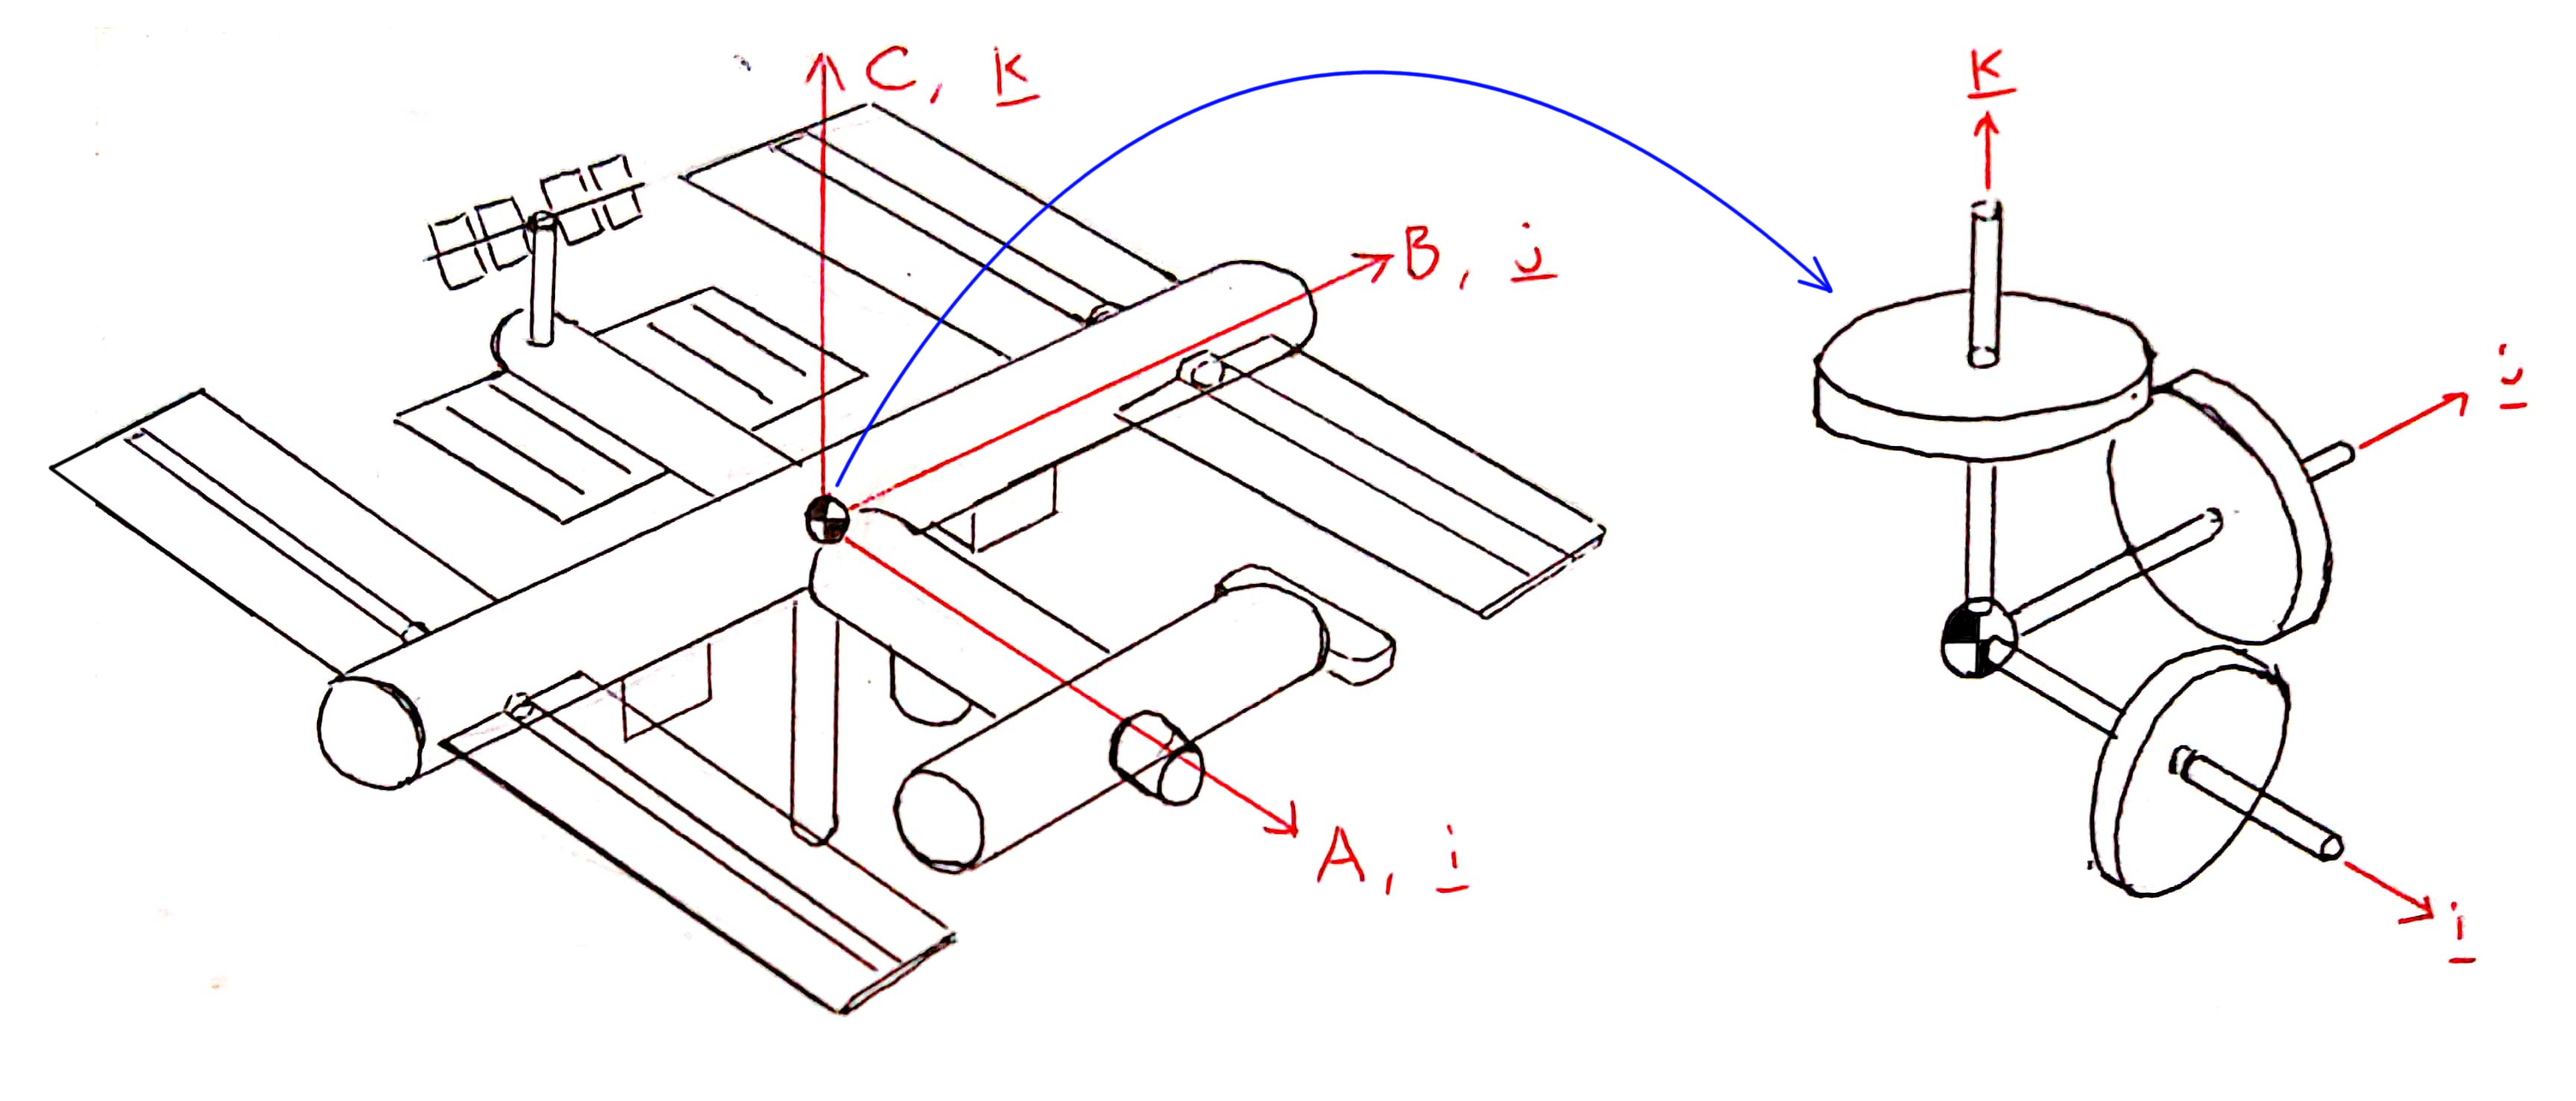
\includegraphics[width=\linewidth]{fig/space_station.png}
\vspace{-0.3cm}
\caption{\label{fig:space_station}Diagram of the space station and attached gyroscopes with principle axis and principle moments of inertia labelled.}
\end{figure}

This modifies the system looked at previously by adding 3 rotors at the centre of mass, aligned with the principle axes. Each gyroscope is an AAC body, with identical moments of inertia $A_R$ and $C_R$ perpendicular to, and along the spin axes. Their inertia matrices are $I_{R1}$, $I_{R2}$ and $I_{R3}$, with the same AAC form, but $C_R$ in different positions.

These moments of inertia are releative to the centre of mass of the spacecraft. These can be related to the moments of inertia about the centre of mass of the rotors $A_{R,G}$ and $C_{R,G}$ by the parallel axis theorem \cite{parallel_axis_theorem}:
\begin{equation} \label{eq:rotor_moments_of_inertia}
C_R = C_{R,G} \quad\quad A_R = A_{R,G} + d^2m
\end{equation}
Where $d$ is the distance along the spin axis from the centre of mass of the rotor to the centre of mass of the spacecraft, and $m$ is the mass of a rotor.

The rotors have spins $\omega_1$, $\omega_2$ and $\omega_3$.

\subsubsection{Equations of Motion}

If the whole spacecraft is rotating with angular velocity $\Omega$ and the reaction wheels are fixed to the spacecraft, then they will be rotating with angular velocities:
\begin{align} \label{reaction_wheel_velocities}
\begin{split}
\textrm{Angular velocity of rotor 1 } &= \bm{\Omega} + \omega_1\bm{i} \\
\textrm{Angular velocity of rotor 2 } &= \bm{\Omega} + \omega_2\bm{j} \\
\textrm{Angular velocity of rotor 3 } &= \bm{\Omega} + \omega_3\bm{k}
\end{split}
\end{align}

Therefore, the total angular momentum, including the spacecraft and rotors can be given by:
\begin{align*}
\bm{h} &= I\bm{\Omega} +
I_{R1}(\bm{\Omega} + \omega_1\bm{i}) +
I_{R2}(\bm{\Omega} + \omega_2\bm{j}) +
I_{R3}(\bm{\Omega} + \omega_3\bm{k}) \\
\bm{h} &= (I + I_{R1} + I_{R2} + I_{R3})\bm{\Omega} +
C_R(\omega_1\bm{i} + \omega_2\bm{j} + \omega_3\bm{k})
\end{align*}
If $I$ is refefined to include the rotor inertia too, then this can be simplified to:
\begin{equation} \label{eq:reaction_wheel_h}
\bm{h} = I\bm{\Omega} + C_R\bm{\omega}
\end{equation}
Where $\bm{\omega}$ is a vector containing the gyroscope spins.

From this, the equations of motion are derived in the same way as before, by using \cref{eq:simple_eq_of_motion} ($\dot{\bm{h}} = 0$) and differentiating $\bm{h}$ in a rotating reference frame using \cref{eq:dif_rotating_frame}. This gives:
\begin{equation} \label{eq:reaction_eq_of_motion_vector}
0 = I\dot{\bm{\Omega}} + C_R\bm{\dot{\omega}} + \bm{\Omega}\times I\bm{\Omega} + C\bm{\Omega}\times \bm{\omega}
\end{equation}

Expanding this out gives the full equations of motion for the reaction wheel system:
\begin{align} \label{eq:reaction_eq_of_motion}
\begin{split}
0 &= A\dot{\Omega}_1 + C_R\dot{\omega}_1 + (C - B)\Omega_2\Omega_3
+ C_R(\Omega_2\omega_3 - \Omega_3\omega_2) \\
0 &= B\dot{\Omega}_2 + C_R\dot{\omega}_2 + (A - C)\Omega_1\Omega_3
+ C_R(\Omega_3\omega_1 - \Omega_1\omega_3) \\
0 &= C\dot{\Omega}_3 + C_R\dot{\omega}_3 + (B - A)\Omega_1\Omega_2
+ C_R(\Omega_1\omega_2 - \Omega_2\omega_1)
\end{split}
\end{align}


\subsubsection{Simple Solutions}

\textbf{The Spacecraft is Stationary}

Setting $\bm{\Omega} = \bm{0}$ gives:
\begin{align*}
0 &= C_R\dot{\omega}_1 \\
0 &= C_R\dot{\omega}_2 \\
0 &= C_R\dot{\omega}_3 \\
\end{align*}
This is a solution if $\bm{\omega}$ is constant. Therefore, if the station has no angular velocity and keeps the rotor spins constant, then it will remain stationary.

\textbf{The Rotors have Zero Spin}

If the rotors have no spin ($\bm{\omega}$=0), then the equations of motion simplify to Euler's equations, shown in \cref{eq:euler_equations}, but with moments of inertia for the combined system instead. Thefefore, the motion is the same as if there were no reaction wheels, as expected.

\subsubsection{Controlling Rotation using a Single Reaction Wheel}

\textbf{Solution for Rotation about a Single Axis}

Setting $\omega_2=0$ and $\omega_3=0$:
\begin{align} \label{eq:reaction_wheel_single_gyro_full}
\begin{split}
0 &= A\dot{\Omega}_1 + C_R\dot{\omega}_1 + (C - B)\Omega_2\Omega_3 \\
0 &= B\dot{\Omega}_2 + (A - C)\Omega_1\Omega_3
+ C_R\Omega_3\omega_1 \\
0 &= C\dot{\Omega}_3 + (B - A)\Omega_1\Omega_2
- C_R\Omega_2\omega_1
\end{split}
\end{align}

Similar to the rotation about a single axis with no reaction wheels, one solution is to have $\Omega_1 = \textrm{Constant}, \Omega_2=0, \Omega_3=0$, giving: 
\begin{align} \label{eq:reaction_wheel_single_gyro_simplified}
\begin{split}
0 &= A\dot{\Omega}_1 + C_R\dot{\omega}_1 \\
0 &= 0 \\
0 &= 0
\end{split}
\end{align}

Therefore:
\begin{align} \label{eq:reaction_wheel_single_gyro_solution}
\begin{split}
\dot{\Omega}_1 &= -\frac{C_R}{A}\dot{\omega}_1 \\
\Delta\Omega_1 &= -\frac{C_R}{A}\Delta\omega_1
\end{split}
\end{align}

This means that if $\omega_1$ is changed then there must be a corresponding change of $\Omega_1$ in the other direction, by conservation of angular momentum.

\textbf{Stability}

Like before, perturbations $\delta\Omega_2$ and $\delta\Omega_3$ can be added, to check the stability of the solution:
\begin{align} \label{eq:reaction_wheel_single_gyro_stability}
\begin{split}
0 &= A\dot{\Omega}_1 + C_R\dot{\omega}_1 \\
0 &= B\dot{\Omega}_2 + (A - C)\Omega_1\dot{\Omega}_3 + C_R\delta\Omega_3\omega_1 \\
0 &= C\dot{\Omega}_3 + (B - A)\Omega_1\dot{\Omega}_2 - C_R\delta\Omega_3\omega_2
\end{split}
\end{align}

This gives the same solution as \cref{eq:euler_stability_solution}, except that the frequency is different:
\begin{equation} \label{eq:reaction_wheel_stability_freq1}
\omega^2 = \frac{1}{BC}[C_R\omega_1 - (C-A)\Omega_1][C_R\omega_1 - (B-A)\Omega_1]
\end{equation}

This expression can be simplified by relating $\omega_1$ and $\Omega_1$ from \cref{eq:reaction_wheel_single_gyro_solution}:
$$ A\dot{\Omega}_1 + C\dot{\omega}_1 = 0 $$
$$ A(\Omega_1 - \Omega_{1,0}) + C_R(\omega_1 - \omega_{1,0}) = 0$$
$$ A\Omega_1 + C_R\omega_1 - h_{1,0} = 0 $$
\begin{equation} \label{eq:reaction_wheel_omega1_sub}
\Omega_1 = - \frac{C_R\omega_1 - h_{1,0}}{A}
\end{equation}

Where $h_{1,0}$ is the intial angular momentum of the system about the $\bm{i}$ axis. For example, this will be non-zero if the rotor is spinning initially.

In the case that $h_{1,0}=0$, substituting \cref{eq:reaction_wheel_omega1_sub} into the expression for $\omega^2$ from \cref{eq:reaction_wheel_stability_freq1} gives:
\begin{equation} \label{eq:reaction_wheel_stability_freq2}
\omega^2 = \left(\frac{C_R\omega_1}{A}\right)^2
\end{equation}

Therefore, if there is no initial angular momentum, then constant angular velocity about a principle axis is always stable, even about an axis with intermediate moment of inertia.

If $h_{1,0} \neq 0$, then the expression becomes more complicated:
\begin{equation} \label{eq:reaction_wheel_stability_freq3}
\omega^2 = \left(\frac{C_R\omega_1}{A}\right)^2
\left[1 - \left(1 - \frac{A}{C}\right)\frac{h_{1,0}}{C_R\omega_1}\right]
\left[1 - \left(1 - \frac{A}{B}\right)\frac{h_{1,0}}{C_R\omega_1}\right]
\end{equation}

\vfill\null
\columnbreak

In this case, the condition for stability depends on the relative size of the moments of inertia and the ratio $h_{1,0}/C_R\omega_1$, so there is no simple rule. However, some observations are:
\begin{itemize}
\item If the gyroscope operates at large spins such that $C_R\omega_1 >> h_{1,0}$, then this is stable.
\item If the space station is an AAA body, then it is always stable.
\item If the moments of inertia are all of similar magnitudes and $h_{1,0}/C_R\omega_1$ doesn't becomes large, then this is always stable.
\end{itemize}

Stability of this solution was investigated with simulated, where \Cref{fig:reaction_single_zero_stable} gives an example of stable motion and \Cref{fig:reaction_single_zero_unstable} gives an example of unstable motion.

\subsection{Controlling Rotation using All Reaction Wheels}

\textbf{Validity of the Solution for a Single Axis Reaction Wheel}

If the initial angular momentum of the spacecraft is zero, then the reaction wheels can rotate about any principle axis by ensuring that the rotor spin and angular velocity along other axes are zero.

The problem with this, is that it is unlikely that the spacecraft has no net angular momentum. Any sort of disturbance will apply an external torque and change angular momentum.

Therefore, it is desirable to come up with a method for rotating about a given axis when the net angular momentum is non-zero. To simplify the analysis, we can start at an initial condition of $\bm{\Omega}=0$, but $\bm{\omega} \neq \bm{0}$ where the reaction wheels have absorbed all the angular momentum.

It can be seen from \cref{eq:reaction_eq_of_motion} that if all the reaction wheel spins are non-zero then the motion becomes unpredictable if attempting to rotate about a single axis by changing a single rotor spin.. \Cref{fig:reaction_naive_attempt} shows an example of what happens if attempting to increase $\Omega_1$ by decreasing $\omega_1$ when the other reaction wheels are spinning too.

Therefore, a solution for changing $\Omega_1$ must involve chaning $\omega_2$ and $\omega_3$ in some way too, not just $\omega_1$.

\vfill\null
\columnbreak

\textbf{Solution for Rotation about a Single Axis when All Reaction Wheels are Spinning}

Take $\bm{\Omega} = \Omega_1\bm{i}$, but allow for $\omega_1$, $\omega_2$ and $\omega_3$ to all vary.
\begin{align} \label{eq:reaction_smart_eq_of_motion}
\begin{split}
0 &= A\dot{\Omega}_1 + C_R\dot{\omega}_1 \\
0 &= B\dot{\Omega}_2 + C_R\dot{\omega}_2 - C_R\Omega_1\omega_3 \\
0 &= C\dot{\Omega}_3 + C_R\dot{\omega}_3 + C_R\Omega_1\omega_2
\end{split}
\end{align}

Here, to keep $\Omega_2$ and $\Omega_3$ at zero, this requires:
\begin{align} \label{eq:reaction_smart_condition}
\begin{split}
C_R\dot{\omega}_2 - C_R\Omega_1\omega_3 &= 0 \\
C_R\dot{\omega}_3 + C_R\Omega_1\omega_2 &= 0
\end{split}
\end{align}

Again, this is a pair of coupled first order equations giving similar solutions to previous equations, except that now the frequency depends on $\Omega_1$ which may vary in time.

If $\Omega_1$ is constant, then the solution is:
\begin{align} \label{eq:reaction_smart_solution1}
\begin{split}
\omega_2 = R\sin{(\Omega_1 t + \phi)} \\
\omega_3 = R\cos{(\Omega_1 t + \phi)}
\end{split}
\end{align}

Where, in order to satisfy initial conditions:
$$ R = \sqrt{\omega_{2,0}^2 + \omega_{3,0}^2} \quad\quad \phi = \arctan{\left(\frac{\omega_{2,0}}{\omega_{3,0}}\right)} $$

If $\Omega_1$ is allowed to change, then the solution is:
\begin{align} \label{eq:reaction_smart_solution2}
\begin{split}
\omega_2 = R\sin{(\theta + \phi)} \\
\omega_3 = R\cos{(\theta + \phi)}
\end{split}
\end{align}

Where $\theta$ is the integral of $\Omega_1$ (the net rotation about $\bm{i}$):
\begin{equation} \label{eq:reaction_smart_solution_theta}
\theta(t) = \int_{\tau=0}^t \Omega_1(\tau) d\tau
\end{equation}

Therefore, this solution is valid even if $\Omega_1$ varies in response to changes in $\omega_1$.

\vfill\null
\columnbreak

\textbf{Intuitive Understanding of this Solution}

\begin{figure}[H]
\centering
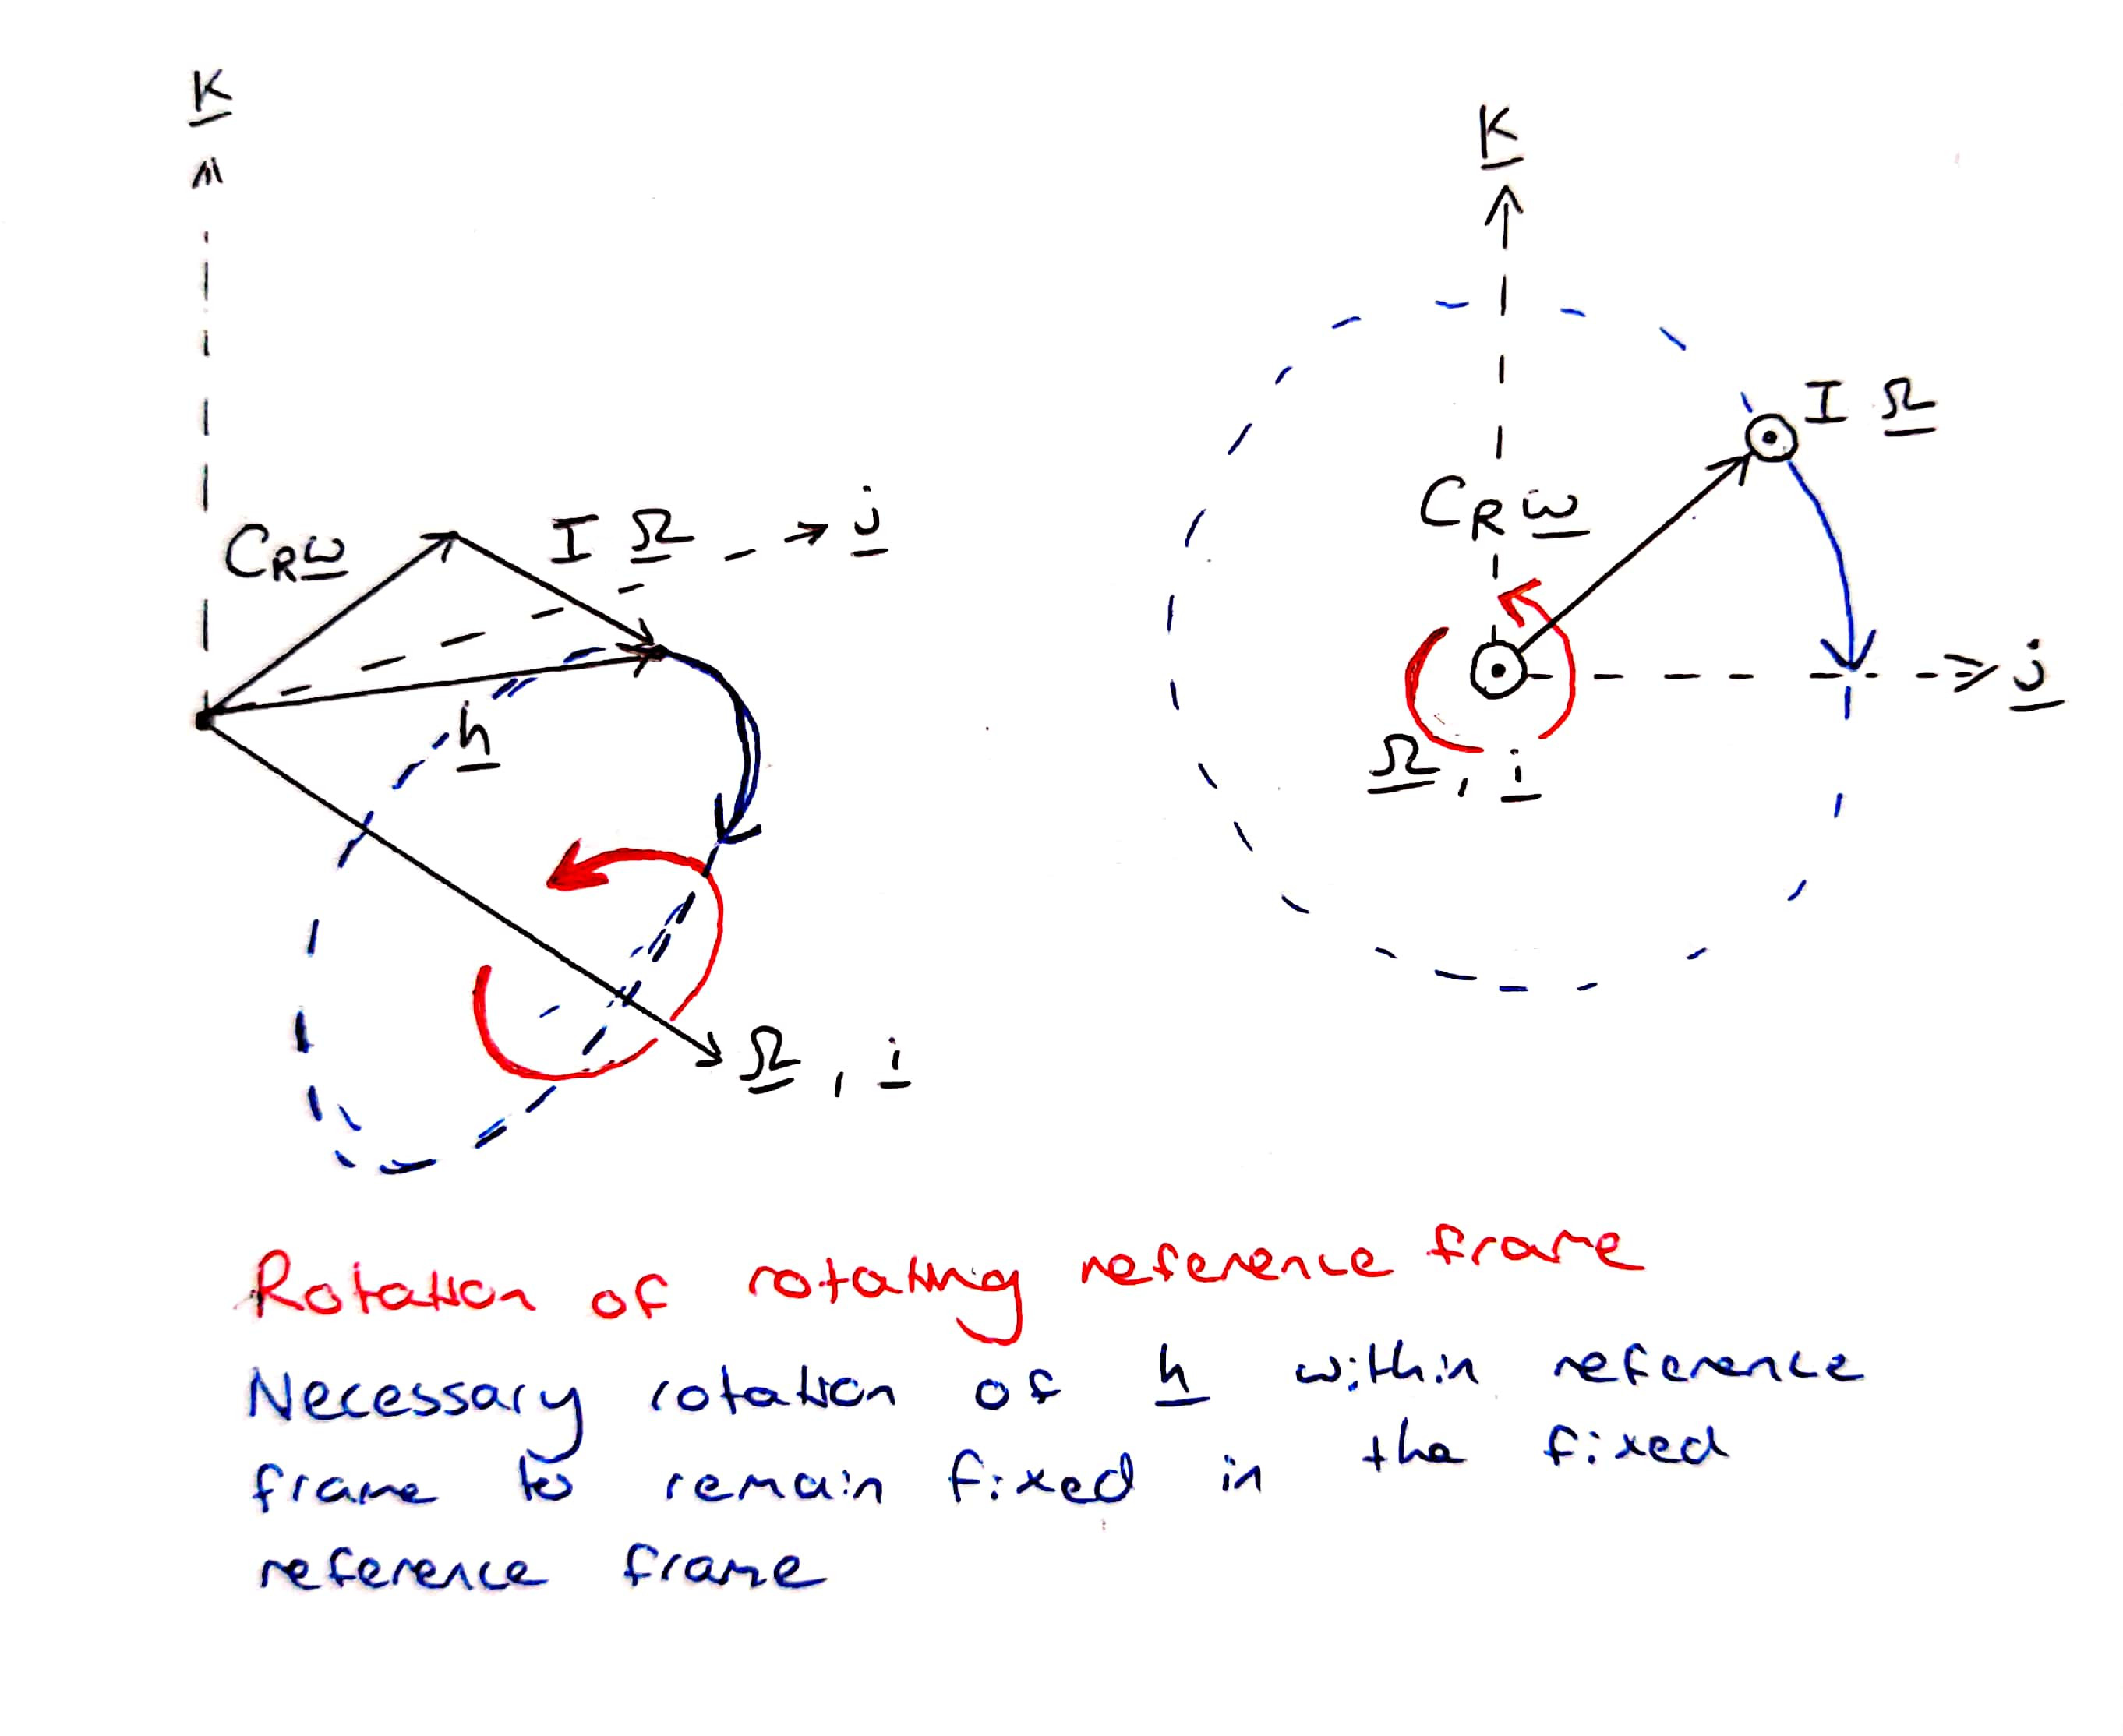
\includegraphics[width=\linewidth]{fig/vector_diagram1.jpg}
\vspace{-0.3cm}
\caption{\label{fig:vector_diagram1}Vector diagram of the angular momentum within the rotating reference frame.}
\end{figure}

\Cref{fig:vector_diagram1} illustrates how the angular momentum must change within the rotating reference frame (aligned with the principle axis of the space station) in order for angular momentum to remain constant in the fixed reference frame. In order to do this, angular momentum must rotate about $\bm{i}$ in the opposite direction to $\Omega_1$. The only quantities which contribute to components of $\bm{h}$ out of the $\bm{i}$ axis are $\omega_2$ and $\omega_3$.

\begin{figure}[H]
\centering
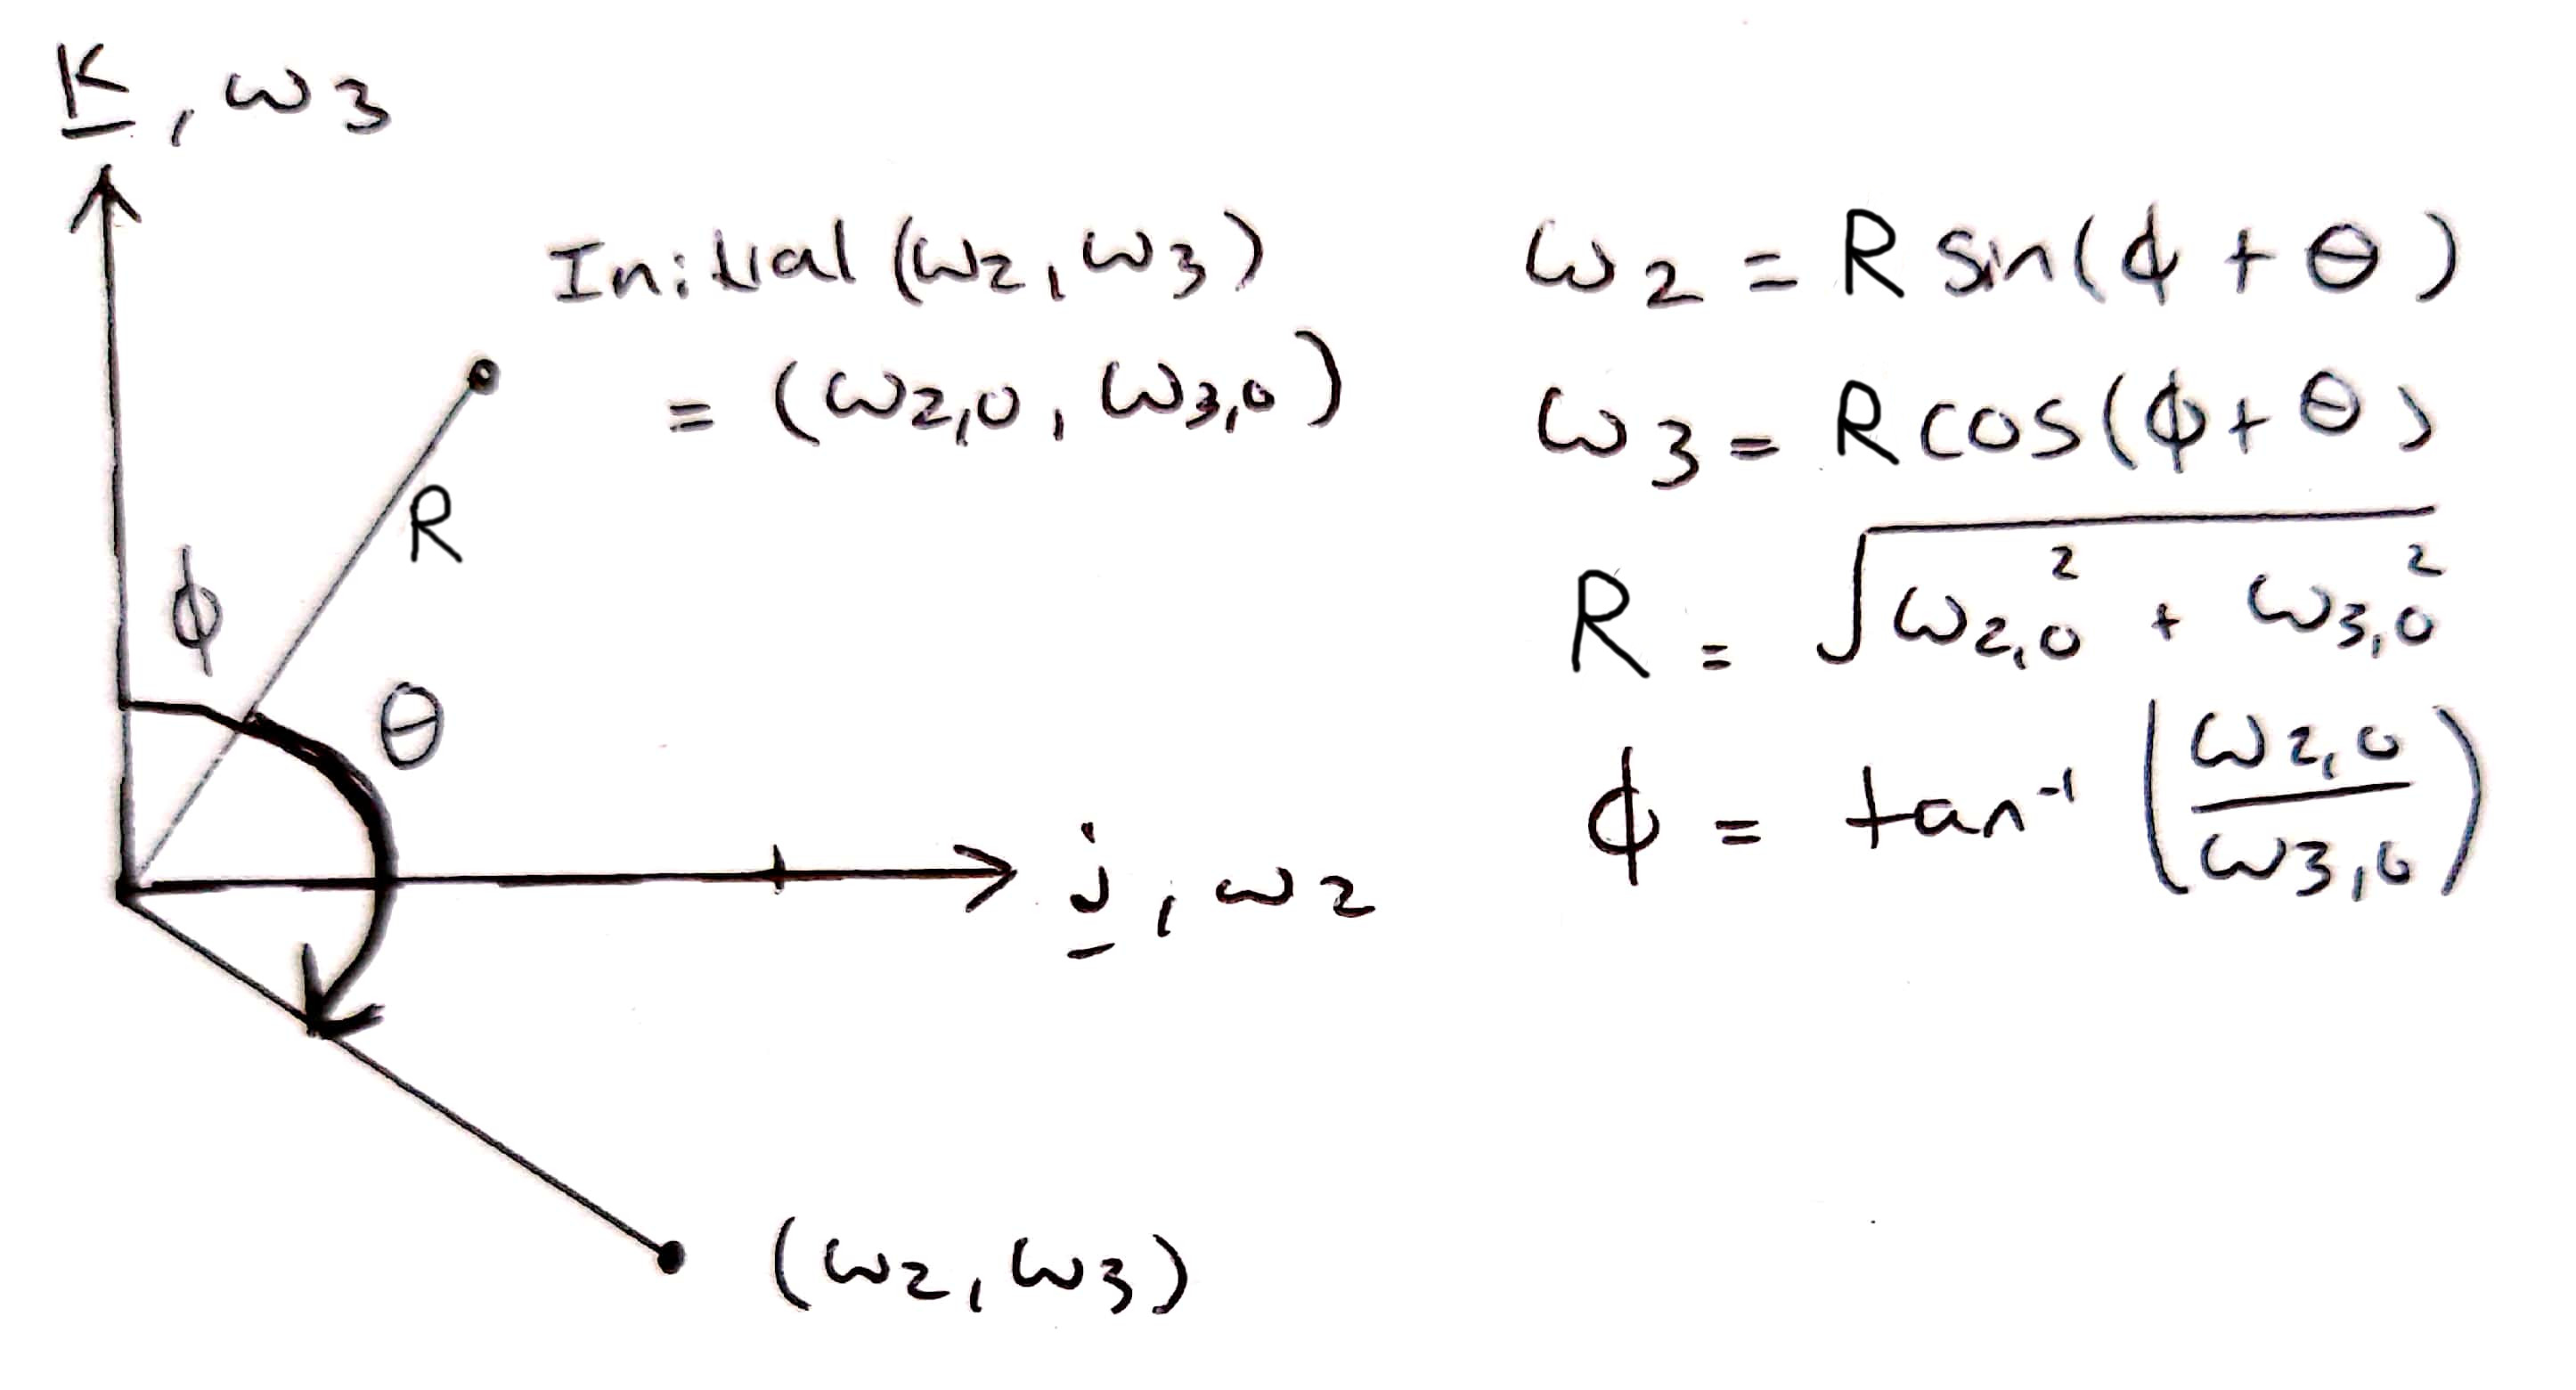
\includegraphics[width=\linewidth]{fig/vector_diagram2.jpg}
\vspace{-0.3cm}
\caption{\label{fig:vector_diagram2}Demonstrates how $\omega_2$ and $\omega_3$ must rotate to counter the rotation from $\Omega_1$.}
\end{figure}

If $(\omega_2, \omega_3)$ must rotate by $\theta = \int\Omega_1 dt$ in the opposite direction of $\Omega_1$, then by geometry, $\omega_2 = R\sin(\phi + \theta)$ and $\omega_3 = R\cos(\phi + \theta)$, where $R$ and $\phi$ depend on the initial conditions as seen before.

\vfill\null
\columnbreak

\textbf{Stability}

Adding perturbations in $\Omega_2$ and $\Omega_3$ to the previous solution gives:
\begin{align} \label{eq:reaction_smart_stability}
\begin{split}
0 &= A\dot{\Omega}_1 + C_R\dot{\omega}_1 +
[C_R(\delta\Omega_2\omega_3 - \delta\Omega_3\omega_2)] \\
0 &= C_R\dot{\omega}_2 - C_R\Omega_1\omega_3 +
[B\dot{\Omega}_2 + (A - C)\Omega_1\dot{\Omega}_3 + C_R\delta\Omega_3\omega_1] \\
0 &= C_R\dot{\omega}_3 - C_R\Omega_1\omega_2 +
[C\dot{\Omega}_3 + (B - A)\Omega_1\dot{\Omega}_2 - C_R\delta\Omega_3\omega_2]
\end{split}
\end{align}
The terms indicated with $[\quad]$ are the new contributions from the perturbations. The solution is identical to the system with a single reaction wheel, where stability requires $\omega^2$ from \cref{eq:reaction_wheel_stability_freq3} to be positive.

The only difference is the extra term in the first line of \cref{eq:reaction_smart_stability} which gives a contribution to $\dot{\Omega}_1$ of:
$$-\frac{C_R}{A}(\delta\Omega_2\omega_3 - \delta\Omega_3\omega_2)$$

Although this term isn't zero, it doesn't change $\Omega_1$ significantly, so can be neglected. However, a more accurate control system could measure $\Omega_2$ and $\Omega_3$ and account for these in the value of $\dot{\omega}_1$ in order to counteract the perturbations.

\subsection{Motion of the Spacecraft with Control Moment Gyroscopes}

\subsubsection{Behavoiur of a Standard Gyroscope}

To give an idea of the effect of the gyroscopes on the spacecraft, it is useful to investigate the behaviour of a standard gyroscope.

The gyroscope looked at is identical to the one in the lab, mounted along an axis through the centre of mass. Gimbal inertia will be ignored, and the rotor has the same moments of inertia as the previous rotors looked at.

The reference frame used will be aligned with the spin axis, with angular velocity $\bm{\Omega}$. The rotor is spinning with a rate of $\omega$ about the $\bm{k}$ axis. Therefore, the angular momentum is given by:
\begin{equation} \label{eq:gyro_h}
\bm{h} = I_R(\bm{\Omega} + \omega\bm{k})
\end{equation}

Differentiating this in a rotating reference frame, and substituting into $\bm{Q} = \dot{\bm{h}}$ gives:
\begin{equation} \label{eq:gyro_eq_of_motion_vector}
\bm{Q} = I_R\dot{\bm{\Omega}} + C_R\dot{\omega}\bm{k} + \Omega \times I_R\Omega + \Omega \times C_R\omega\bm{k}
\end{equation}

Which when expanded out, gives:
\begin{align} \label{eq:gyro_eq_of_motion}
\begin{split}
Q_1 &= A_R\dot{\Omega}_1 + [(C_R-A_R)\Omega_3 + C_R\omega]\Omega_2 \\
Q_2 &= A_R\dot{\Omega}_2 - [(C_R-A_R)\Omega_3 + C_R\omega]\Omega_1 \\
Q_3 &= C_R(\dot{\Omega}_3 + \dot{\omega}) \\
\end{split}
\end{align}

Since the gyroscopes will be operating with large rotor spin, $C_R\omega >> (C_R-A_R)\Omega_3$, this can be simplified to:
\begin{align} \label{eq:gyro_eq_of_motion_fast_spin}
\begin{split}
Q_1 &= A_R\dot{\Omega}_1 + C_R\omega\Omega_2 \\
Q_2 &= A_R\dot{\Omega}_2 - C_R\omega\Omega_1 \\
Q_3 &= C_R(\dot{\Omega}_3 + \dot{\omega}) \\
\end{split}
\end{align}

\textbf{Using Euler Angles}

\begin{figure}[H]
\centering
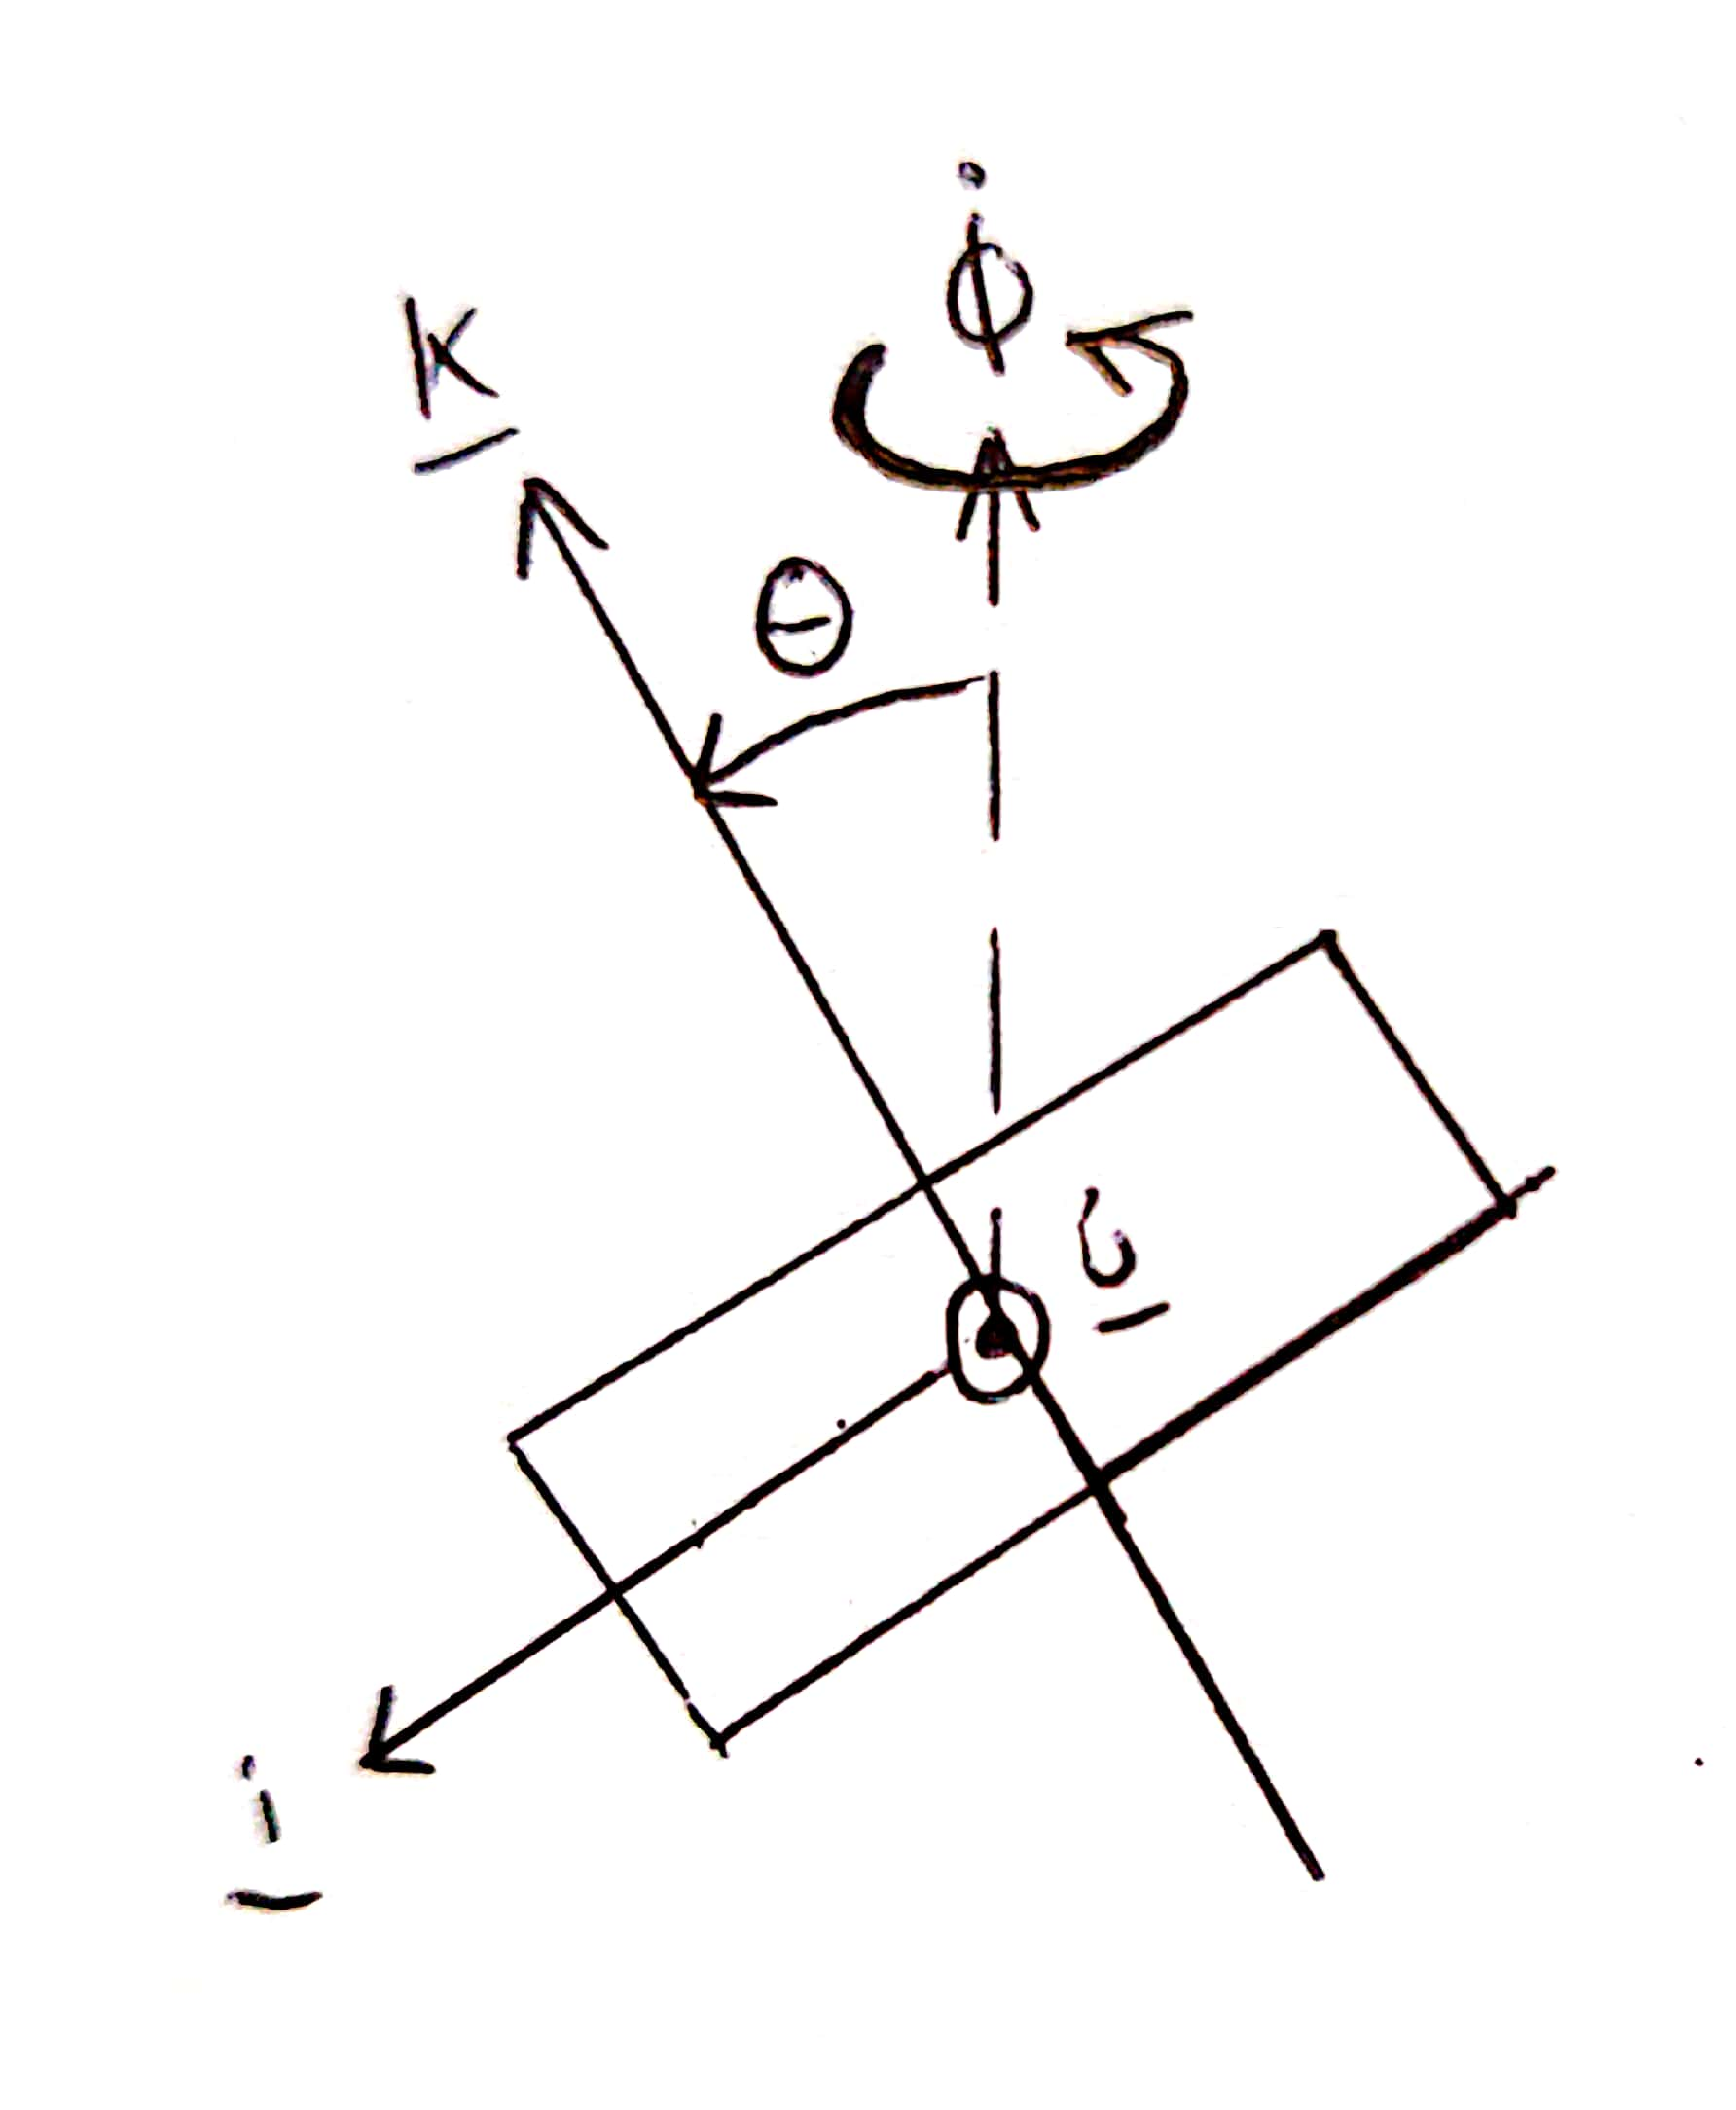
\includegraphics[width=0.6\linewidth]{fig/euler_angles.jpg}
\vspace{-0.3cm}
\caption{\label{fig:euler_angles}Description of gyroscope spin axis using Euler angles.}
\end{figure}

If the spin axis is described in terms of euler angles as shown in \Cref{fig:euler_angles}, then $\bm{\Omega}$ is equal to:
\begin{equation}
\bm{\omega} =
\begin{pmatrix}
-\dot{\phi}\sin{\theta} \\
\dot{\omega} \\
\dot{\phi}\cos{\theta}
\end{pmatrix}
\end{equation}

Substituting this into \cref{eq:gyro_eq_of_motion_fast_spin} gives:
\begin{align} \label{eq:gyro_eq_of_motion_euler}
\begin{split}
Q_1 &= -A_R(\ddot{\phi} + \dot{\phi}\dot{\theta}\cos\theta) + C_R\omega\dot{\theta} \\
Q_2 &= A_R\dot{\theta} + C_R\omega\dot{\phi}\sin\theta \\
Q_3 &= C_R(\ddot{\phi}\cos\theta - \dot{\phi}\dot{\theta}\sin\theta + \dot{\omega}) \\
\end{split}
\end{align}

\textbf{Equilibrium Solution with an Applied Couple}

If no couple is applied to the system, then it will remain stationary. However, if a couple $Q_2$ is applied then line 2 of \cref{eq:gyro_eq_of_motion_euler} gives:
\begin{equation}
Q_2 = C_R\omega\dot{\phi}\sin\theta
\end{equation}

Therefore, the precession rate is constant and depends on the applied couple, rotor spin and spin axis inclination:
\begin{equation} \label{eq:gyro_precession_rate}
\dot{\phi} = \frac{Q_2}{C_R\omega\sin\theta}
\end{equation}

By attaching these gyroscopes to a spacecraft, the phenomenon of precession can be utilised to rotate the spacecraft.

\subsubsection{Structure of the Control Moment Gyroscope System}

The structure of the control moment gyroscope system is similar to the reaction wheel system, except that instead of varying the spin of the rotors, the spin axes are tilted instead.

\begin{figure}[H]
\centering
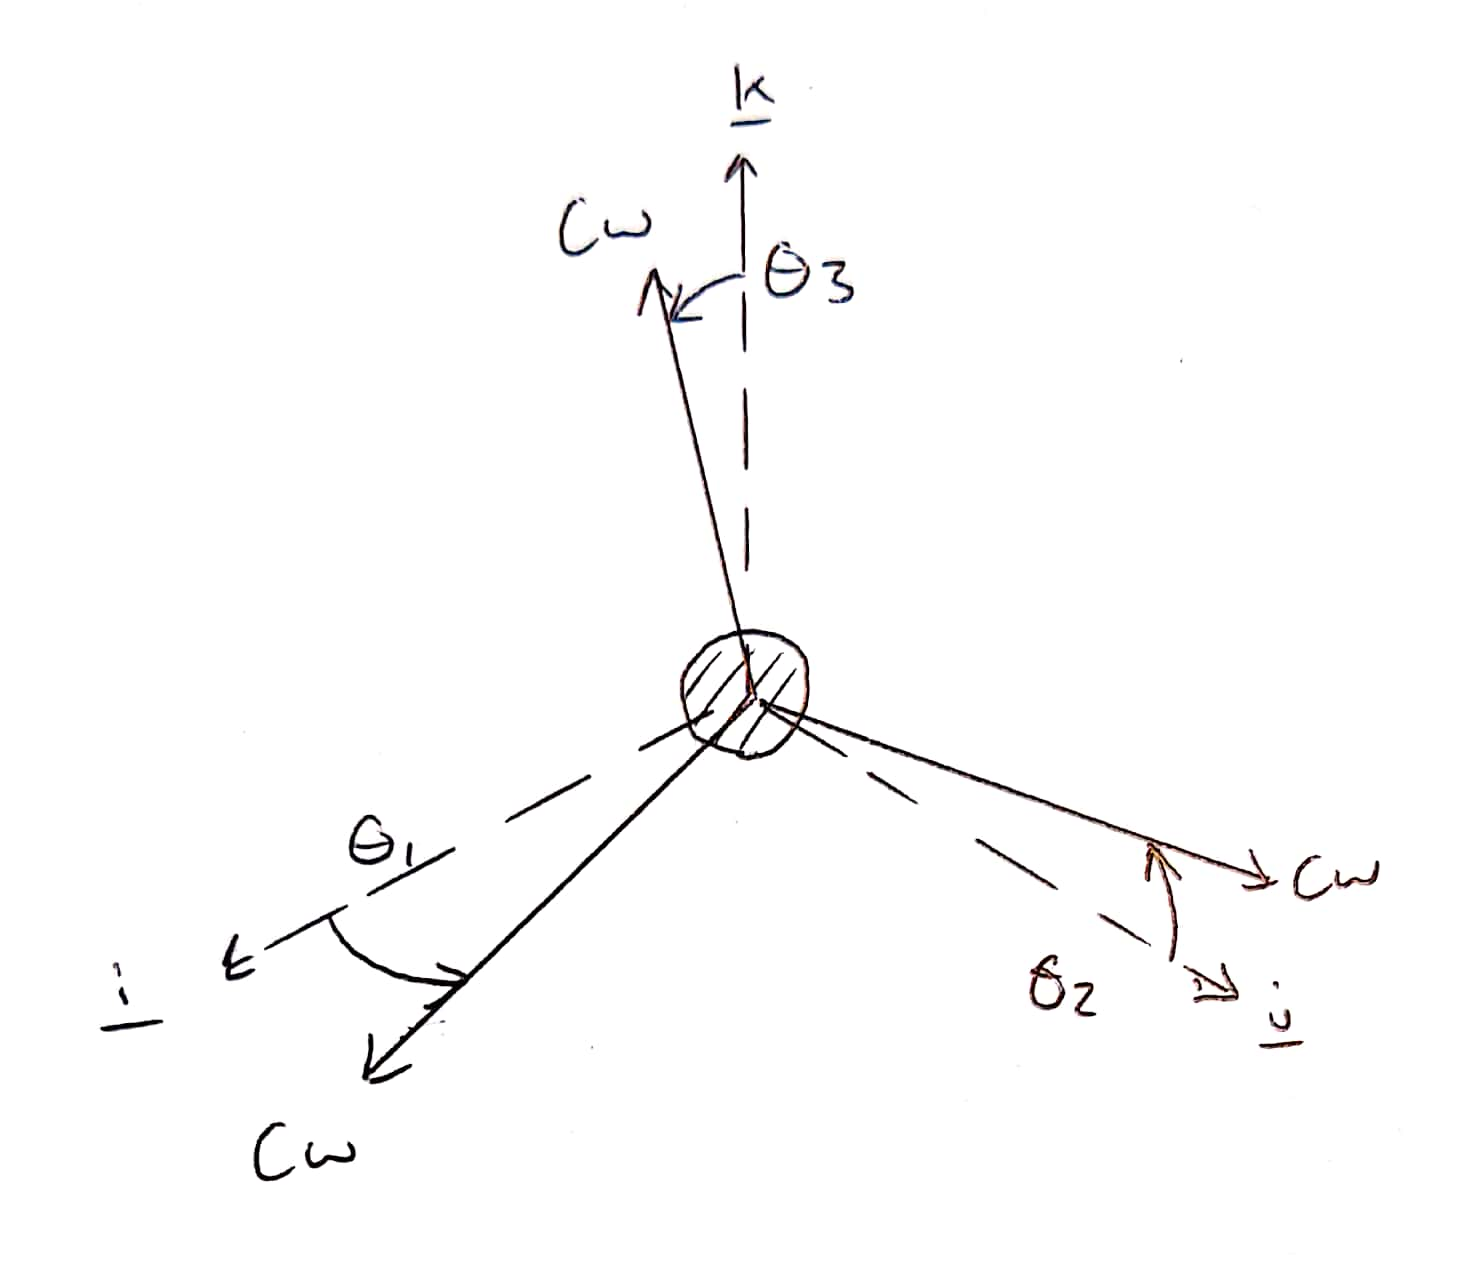
\includegraphics[width=0.6\linewidth]{fig/cmg_diagram.jpg}
\vspace{-0.3cm}
\caption{\label{fig:cmg_diagram}Description of control moment gyroscope system, with inclination of spin axes labelled.}
\end{figure}

The rotors have identical, constant spin $\omega$. The gyroscopes are mounted in single-gimbals such that each rotor axis is able to tilt in a single direction. The inclinations are $\theta_1$, $\theta_2$ and $\theta_3$, each about a different axis.

\subsubsection{Equations of Motion}

The total moment of inertia can be given by \cref{eq:cmg_h} below:
\begin{equation} \label{eq:cmg_h}
\bm{h} = I\bm{\Omega} +
C_R\omega\begin{pmatrix}
\cos\theta_1 + \sin\theta_3 \\
\cos\theta_2 + \sin\theta_1 \\
\cos\theta_3 + \sin\theta_2
\end{pmatrix}
\end{equation}

In deriving this, it has been assumed that the angular momentum of the rotors can neglect the contribution from the rotation $\bm{\Omega}$ of the spacecraft. This is sensible, since the spacecraft will have much larger moments of inertia than the rotor. Therefore the angular momentum of the rotors $C_R\omega$ can simply be mapped onto the principle axes of the spacecraft.

Differentiating this in a rotating reference frame using \cref{eq:dif_rotating_frame} and substituting into \cref{eq:simple_eq_of_motion} ($\bm{Q} = \dot{h} = 0$) will give the equations of motions. To simplify this equation to something more useful, it can be assumed that the inclination angles are small and second order terms can be ignored, giving:
\begin{align} \label{eq:cmg_eq_of_motion}
\begin{split}
0 &= A\dot{\Omega}_1 + (C-B)\Omega_2\Omega_3 + C_R\omega\dot{\theta}_3 + C_R\omega(\Omega_2 - \Omega_3) \\
0 &= B\dot{\Omega}_2 + (A-C)\Omega_1\Omega_3 + C_R\omega\dot{\theta}_1 + C_R\omega(\Omega_3 - \Omega_1) \\
0 &= C\dot{\Omega}_3 + (B-A)\Omega_1\Omega_2 + C_R\omega\dot{\theta}_2 + C_R\omega(\Omega_1 - \Omega_2)
\end{split}
\end{align}

\subsubsection{Controlling Rotation}

To get an idea of the behaviour of the system, the initial behaviour when starting from rest can be considered, where $\bm{\Omega} = \bm{0}$. This gives:
\begin{align} \label{eq:cmg_initial}
\begin{split}
0 &= A\dot{\Omega}_1 + C_R\omega\dot{\theta}_3 \\
0 &= B\dot{\Omega}_2 + C_R\omega\dot{\theta}_1 \\
0 &= C\dot{\Omega}_3 + C_R\omega\dot{\theta}_2
\end{split}
\end{align}

Therefore, by changing the inclination of one of the axis, this will change the angular velocity of the body about another axis. For example, $\Omega_1$ is controlled by $\theta_3$ according to:
\begin{align} \label{eq:cmg_solution}
\begin{split}
\dot{\Omega}_1 &= -\frac{C_R}{A}\dot{\theta}_3 \\
\Delta\Omega_1 &= -\frac{C_R}{A}\Delta\theta_3 + \textrm{Constant}
\end{split}
\end{align}

However, once $\Omega_1$ becomes non-zero, this changes the solution:
\begin{align} \label{eq:cmg_steady_behaviour}
\begin{split}
0 &= A\dot{\Omega}_1 + C_R\omega\dot{\theta}_3 \\
0 &= B\dot{\Omega}_2 + C_R\omega\dot{\theta}_1 - C_R\omega\Omega_1 \\
0 &= C\dot{\Omega}_3 + C_R\omega\dot{\theta}_2 + C_R\omega\Omega_1
\end{split}
\end{align}

Once $\Omega_1$ is non-zero, this causes $\Omega_2$ and $\Omega_3$ to change. From \cref{eq:cmg_solution} and \cref{eq:cmg_steady_behaviour}, assuming that both $\Omega_1$ and $\theta_1$ were initally zero, this gives:
\begin{align} \label{eq:cmg_other_rotation}
\begin{split}
\dot{\Omega}_2 &= \frac{C_R\omega}{B}\Omega_1 = -\frac{C_R^2\omega}{AB}\theta_3 \\
\dot{\Omega}_3 &= -\frac{C_R\omega}{C}\Omega_1 = \frac{C_R^2\omega}{AC}\theta_3 \\
\end{split}
\end{align}

If $AB>>C_R^2\omega$ and $AC>>C_R^2\omega$ then these angular velocities can be made small, but will not be zero. Therefore, this method of controlling the spacecraft motion can only be active for short periods of time while $\Omega_2$ and $\Omega_3$. If these angular velocities become large, the motion will become unpredictable. Alternatively, more complex control methods could be designed to counter these off-axis angular velocities.

\Cref{fig:cmg_controlled} and \Cref{fig:cmg_uncontrolled} show a controlled and uncontrolled change in attitude by attempting to rotate about a single axis.

\subsubsection{Comparison with a Standard Gyroscope}

The control moment gyroscopes utilise precession to rotate the spacecraft body, in the same way that a gyroscope will undergo precession if an external couple is applied. When the spin axis of a rotor is tilted, in order to keep the net angular momentum constant, the whole system must increase its angular momentum in the opposite direction to this, which is done by rotating the system using precessoin

In order to tilt the axis, a couple must be applied to the CMG. When considering the whole system together, this is an internal couple so doesn't appear in the equations of motion. However, if the spacecraft and CMG were viewed separately, this would show that when the spacecraft applies a couple to rotate the spin axis, an equal and opposite couple is exerted on the spacecraft, accelerating it and causing it to start precessing.

\section{Conclusions}

\begin{enumerate}
\item For an ABC body, motion about a principle axis is stable if the corresponding moment of inertia is a minimum or maximum, but unstable if it is the intermediate one.
\item Both reaction wheels and control moment gyroscopes use conservation of angular momentum to manipulate the angular velocity of the spacecraft. Reaction wheels do this by changing the spin of rotors with fixed spin axes, while control moment gyroscopes do this by tilting the spin axis of rotors, which have  constant spin.
\item If using a single reaction wheel, the attitude control method is simple. Any change in the angular momentum of the wheel will produce an equal and opposite change in the angular momentum of the spacecraft. This solution is stable for most situations, becoming unstable when rotating about the spacecraft intermediate axis with a large initial angular momentum about this axis.
\item If using multiple reaction wheels, the attitude control method needs to be modified to vary the spin of the other two reaction wheels to counteract the rotation of the spacecraft and keep angular momentum constant.
\item For control moment gyroscopes, tilting the spin axis will produce rotation along an axis perpendicular to the spin axis, by precession. This method requiers that precession occurs for a short period of time. If not, angular velocity is produced in the other two axes, causing the motino to become uncontrolled.
\end{enumerate}

\vfill\null
\columnbreak

\begin{thebibliography}{9}

\bibitem{reaction_wheels}
Fraser Cain,
13/08/19,
\textit{Spacecraft Gyroscopes and Reaction Wheels. You Can Never Have Enough} \\
https://www.universetoday.com/143152/spacecraft-gyroscopes-and-reaction-wheels-you-can-never-have-enough/ (Accessed: 05/12/19)

\bibitem{hubble}
Nasa, \textit{Hubble Space Telescope - Pointing Control System} \\
https://www.nasa.gov/content/goddard/hubble-space-telescope-pointing-control-system (Accessed: 05/12/19)

\bibitem{device_explanation}
Karthikeyan KC,
03/08/16,
\textit{How Reaction Wheels and Control Moment Gyros Work?} \\
https://geekswipe.net/technology/aerospace/how-reaction-wheels-and-control-moment-gyros-work/ \\(Accessed: 05/12/19)

\bibitem{RK4}
Erik Cheever, \textit{Fourth Order Runge-Kutta} \\
https://lpsa.swarthmore.edu/NumInt/NumIntFourth.html (Accessed: 06/12/19)

\bibitem{inertia_matrix}
Meriam J.L., Kraige L.G., 2012, \textit{Engineering Mechanics: Dynamics, 7th edition}, Chapter 7, pp.541

\bibitem{Q_equals_hdot}
Meriam J.L., Kraige L.G., 2012, \textit{Engineering Mechanics: Dynamics, 7th edition}, Chapter 4, pp.274, equation (4/11)

\bibitem{dif_rotating_frame}
Meriam J.L., Kraige L.G., 2012, \textit{Engineering Mechanics: Dynamics, 7th edition}, Chapter 7, pp.527, equation (7/4)

\bibitem{parallel_axis_theorem}
Meriam J.L., Kraige L.G., 2012, \textit{Engineering Mechanics: Dynamics, 7th edition}, Appendix B, pp.643, equation (B/3)

\end{thebibliography}

\end{multicols*}

\section{Appendix}

\subsection{Code for Integrating the Equations of Motion for The Spacecraft with No Actuation Devices}

\inputminted{python}{code/files/no_actuation.py}

\subsection{Code for Integrating the Equations of Motion for The Spacecraft with Reaction Wheels}

\inputminted{python}{code/files/reaction.py}

\vfill\null

\subsection{Code for Integrating the Equations of Motion for The Spacecraft with Control Moment Gyroscopes}

\inputminted{python}{code/files/cmg.py}

\end{document}